%%%%%%%%%%%%%%%%%%%%%%%%%%%%%%%%%%%%%%%%%
% Short Sectioned Assignment LaTeX Template Version 1.0 (5/5/12)
% This template has been downloaded from: http://www.LaTeXTemplates.com
% Original author:  Frits Wenneker (http://www.howtotex.com)
% License: CC BY-NC-SA 3.0 (http://creativecommons.org/licenses/by-nc-sa/3.0/)
%%%%%%%%%%%%%%%%%%%%%%%%%%%%%%%%%%%%%%%%%

%----------------------------------------------------------------------------------------
%	PACKAGES AND OTHER DOCUMENT CONFIGURATIONS
%----------------------------------------------------------------------------------------

\documentclass[paper=a4, fontsize=11pt]{scrartcl} % A4 paper and 11pt font size

% ---- Entrada y salida de texto -----

\usepackage[T1]{fontenc} % Use 8-bit encoding that has 256 glyphs
\usepackage[utf8]{inputenc}
%\usepackage{fourier} % Use the Adobe Utopia font for the document - comment this line to return to the LaTeX default

% ---- Idioma --------

\usepackage[spanish, es-tabla]{babel} % Selecciona el español para palabras introducidas automáticamente, p.ej. "septiembre" en la fecha y especifica que se use la palabra Tabla en vez de Cuadro

% ---- Otros paquetes ----

\usepackage{amsmath,amsfonts,amsthm} % Math packages
%\usepackage{graphics,graphicx, floatrow} %para incluir imágenes y notas en las imágenes
\usepackage{graphics,graphicx, float, url} %para incluir imágenes y colocarlas

% Para hacer tablas comlejas
%\usepackage{multirow}
%\usepackage{threeparttable}
\usepackage{float}


%\usepackage{sectsty} % Allows customizing section commands
%\allsectionsfont{\centering \normalfont\scshape} % Make all sections centered, the default font and small caps

\usepackage{fancyhdr} % Custom headers and footers
\pagestyle{fancyplain} % Makes all pages in the document conform to the custom headers and footers
\fancyhead{} % No page header - if you want one, create it in the same way as the footers below
\fancyfoot[L]{} % Empty left footer
\fancyfoot[C]{} % Empty center footer
\fancyfoot[R]{\thepage} % Page numbering for right footer
\renewcommand{\headrulewidth}{0pt} % Remove header underlines
\renewcommand{\footrulewidth}{0pt} % Remove footer underlines
\setlength{\headheight}{13.6pt} % Customize the height of the header

\numberwithin{equation}{section} % Number equations within sections (i.e. 1.1, 1.2, 2.1, 2.2 instead of 1, 2, 3, 4)
\numberwithin{figure}{section} % Number figures within sections (i.e. 1.1, 1.2, 2.1, 2.2 instead of 1, 2, 3, 4)
\numberwithin{table}{section} % Number tables within sections (i.e. 1.1, 1.2, 2.1, 2.2 instead of 1, 2, 3, 4)

\setlength\parindent{0pt} % Removes all indentation from paragraphs - comment this line for an assignment with lots of text

\newcommand{\horrule}[1]{\rule{\linewidth}{#1}} % Create horizontal rule command with 1 argument of height


\title{	
	\normalfont \normalsize 
	\textsc{{\bf Ingeniería de Servidores (2014-2015)} \\ Grado en Ingeniería Informática \\ Universidad de Granada} \\ [25pt] % Your university, school and/or department name(s)
	\horrule{0.5pt} \\[0.4cm] % Thin top horizontal rule
	\huge Memoria Práctica 2 \\ % The assignment title
	\horrule{2pt} \\[0.5cm] % Thick bottom horizontal rule
}

\author{Iván Sevillano García} % Nombre y apellidos

\date{\normalsize\today} % Incluye la fecha actual

\begin{document}

\maketitle % Muestra el Título

\newpage %inserta un salto de página

\tableofcontents % para generar el índice de contenidos

\newpage

\section{Instalación de servicios y configuraciones.}
En esta sección se responden a las preguntas referentes a la administración y configuración de software en los distintos sistemas operativos.
\subsection{Yum. Gestor de paquetes de CentOS.}

Esta aplicación es el gestor predeterminado de CentOS, Red Hat, Fedora y derivados.

\begin{itemize}
	\item \textbf{Liste los argumentos de yum necesarios para instalar, buscar y eliminar paquetes.}\\
	Según el manual de yum\cite{yum}, para instalar un paquete del que ya sabemos el nombre podremos utilizar yum seguido del comando \textbf{install} tras el que pondremos el paquete a instalar. También existe la orden \textbf{groupinstall}, que instala un grupo de paquetes de forma conjunta. En realidad funciona igual que la orden install junto al nombre de todos los paquetes del grupo.\\
	
	Para buscar, el comando \textbf{search} seguido de alguna referencia indirecta del paquete(parte del nombre en general) nos dará como resultado los paquetes que tengan algo que ver con la clave de búsqueda.\\
	
	Para eliminar paquetes, yum tiene comandos \textbf{remove} y \textbf{erase} seguidos del paquete a eliminar, lo que produce redundancia de funciones, ya que hacen exactamente el mismo trabajo. Esto es un fallo de diseño y se deberá eliminar uno de estos términos en un futuro.\\
	
	\item \textbf{¿Que hay que hacer para que yum tenga acceso a internet en el aula de prácticas(puesto que esta utiliza un proxy por detrás)?}\\
	
	Para contestar a esta pregunta se nos ofrece dos pistas: acceder al archivo de configuración de yum en /etc/yum/ y que el proxy a utilizar es \textbf{stargate.ugr.es:3128}. Buscamos en el manual de configuración de yum\cite{yum.conf} y nos dice que necesitamos incluir en el archivo \textbf{yum.conf} la URL del proxy. También hay opciones para acceder al proxy con un usuario y una contraseña(proxy\_username y proxy\_password).
	
\end{itemize}

\subsection{Apt. Gestor de paquetes de Debian.}
Esta aplicación es el gestor predeterminado de Debian y sus derivados, como por ejemplo ubuntu.
\begin{itemize}
	\item \textbf{Indique el comando para buscar un paquete en un repositorio y el correspondiente para instalarlo.}\\
	Según el manual de apt\cite{apt}, para buscar un paquete del que tenemos parte del nombre o similar, debemos utilizar el comando \textbf{apt search}, y para instalarlo, el comando \textbf{apt install}.\cite{b1}
	
	
	 \item \textbf{Indique qué ha modificado para que apt pueda acceder a los servidores de paquetes a través del proxy. ¿Cómo añadimos un nuevo repositorio?}\\
	 Según el manual proporcionado por apt.conf\cite{apt.conf}:\\
	 
	 "\textit{http::Proxy define el proxy predeterminado que utilizar para direcciones HTTP URI. Utiliza el formato estándar
	 	http://[[usuario][:contraseña]@]máquina[:puerto]/. También se puede especificar un proxy por cada máquina usando la forma
	 	http::Proxy::<máquina> con la palabra especial DIRECT que significa que no se use ningún proxy. La variable de entorno http\_proxy
	 	se usará en caso de no definir ninguna de las opciones anteriores.
	 }"\\
	 
	 También según el mismo manual, la forma de añadir repositorios es añadirlos al archivo /etc/apt/sources.list con permisos de root. Se puede utilizar el comando edit-sources, con el mismo resultado que editarlos con un editor de texto directamente, ya que este comando solo llama a un editor a escoger\cite{apt}.
	 
\end{itemize}

\subsection{Cuestión opcional: Gestor de paquetes de OpenSUSE.}
Por cuestión de tiempo, en esta asignatura no utilizaremos OpenSUSE, pero si vamos a responder a la pregunta de cuál es el gestor de paquetes de este Sistema Operativo.\\

En la página oficial de OpenSUSE\cite{opensuse}, se dice que éste tiene dos gestores, uno con un entorno gráfico y otro para consola. El primero es YaST y el segundo, Zypper.

\newpage
\section{Instalación del servicio de acceso seguro(SSH)}
 
 Para el acceso remoto desde una máquina a otra hay distintos protocolos. Entre ellos, destacan telnet y ssh. Sin embargo, para las conexiones que realizaremos, utilizaremos ssh. La instalación del servidor en Ubuntu se realiza con el comando:\\
 
 $sudo$ $apt$ $install$ $openssh$-$server$\\
 
 
 \begin{itemize}
 	\item ¿Cuál es la diferencia entre telnet y ssh?\\
 	Telnet es un servicio básico de conexión entre máquinas, en el cuál sólo hay envío y recepción de mensajes. Ssh (Secure shell), además de esto, los mensajes se envían de forma segura mediante distintos métodos, como pueden ser la encriptación de información. En definitiva, ssh está varios niveles por encima de telnet. Usar ssh en las prácticas es esencial ya que es mucho mas completo.
 	
 	\item ¿Para qué sirve la opción -X de ssh? Ejecute remotamente, es decir, desde la máquina anfitriona (si tiene Linux) o desde la otra máquina virtual, el comando gedit en una sesión abierta con ssh. ¿Qué ocurre?\\
 	
 	La opción -X habilita la interfaz gráfica en las sesiones ssh. Sin embargo, para que esto tenga sentido, la interfaz gráfica tiene que estar instalada en ambas máquinas, además de que el servidor tiene que aceptar en su archivo de configuración\cite{ssh_config} la posibilidad de utilizar 
 	
 \end{itemize}
 
 Tras instalar el servicio openssh-server en la máquina, probaremos ahora a conectarnos remotamente. Sin embargo, como vemos a continuación, la máquina anfitrión nos pide una contraseña(la contraseña de la cuenta):\\
 
 \begin{figure}[H]
	\centering
	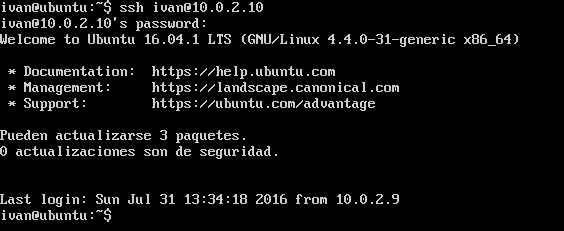
\includegraphics[width=0.7\linewidth]{ssh_no_clave}
	\caption[Sesión ssh]{}
	\caption{}
	\label{fig:ssh_no_clave}
\end{figure}

Sin embargo, esta conexión puede ser insegura. Para hacerla más segura, vamos a utilizar el algoritmo RSA. Para ello generaremos una clave pública en el cliente que enviaremos al servidor. Con esto conseguimos que cada vez que intentemos conectarnos al servidor, no nos pregunte la contraseña de la cuenta del servidor. Esta es la secuencia de operaciones:\\

\begin{figure}[H]
	\centering
	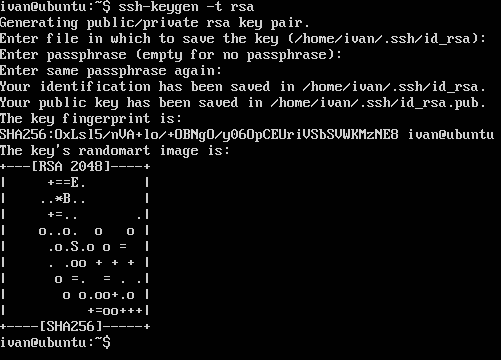
\includegraphics[width=0.7\linewidth]{keygen}
	\caption[Generando clave]{Comando ssh-keygen generando clave RSA}
	\label{fig:keygen}	
\end{figure}

En esta imagen se muestra cuales son los pasos a seguir para generar con ssh-keygen la clave. Según el manual de ssh-keygen\cite{ssh-keygen}, hay muchas opciones, pero la que nos interesa a nosotros es la opción -$t$, que especifica el protocolo que usaremos. Tras esto, keygen nos pregunta que si queremos ponerle una clave, que no será la clave pública, si no una clave interna de paso del ordenador que no pasará a la red. Nos pregunta también por donde guardar la clave. Dejaremos que la guarde por defecto en $/home/ivan/.ssh/id_rsa.pub$. \\

El siguiente paso será enviar la clave pública al servidor para que nos identifique:

\begin{figure}[H]
	\centering
	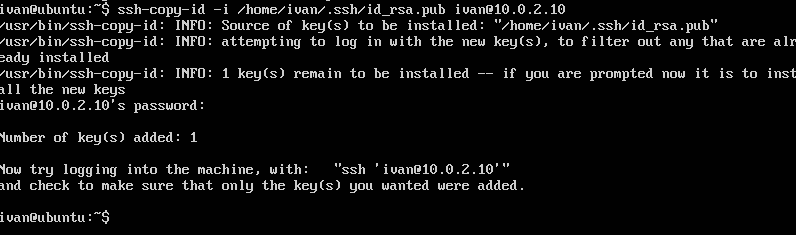
\includegraphics[width=0.7\linewidth]{ssh-copy-id}
	\caption[Uso de copy-id]{Envío de clave pública mediante ssh-copy-id}
	\label{fig:ssh-copy-id}
\end{figure}
 
Según el manual de ssh-copy-id\cite{copy-id}, la forma de uso es indicando la clave pública, con la opción -i, y el servidor ssh. Las últimas líneas de información nos dicen que ya está configurado para poder acceder a la cuenta con la clave pública. Probamos ahora a conectarnos.



 


\newpage
\begin{thebibliography}{xx}
	\bibitem{yum} http://linux.die.net/man/8/yum
	\bibitem{yum.conf} http://linux.die.net/man/5/yum.conf
	\bibitem{apt} http://linux.die.net/man/8/apt
	\bibitem{apt.conf} http://linux.die.net/man/5/apt.conf
	\bibitem{yast} https://es.opensuse.org
	\bibitem{telnet} http://linux.die.net/man/1/telnet
	\bibitem{ssh-client} http://linux.die.net/man/1/ssh
	\bibitem{ssh-keygen} http://linux.die.net/man/1/ssh-keygen
	\bibitem{copy-id} http://linux.die.net/man/1/ssh-copy-id
	
\end{thebibliography}
\end{document}